\section{Introduction} % Seções são adicionadas para organizar sua apresentação em blocos discretos, todas as seções e subseções são automaticamente exibidas no índice como uma visão geral da apresentação, mas NÃO são exibidas como slides separados.

%----------------------------------------------------------------------------------------

\begin{frame}
\frametitle{Introduction}
\begin{columns}
        % First column
        \begin{column}{0.5\textwidth}
     \begin{itemize}
         \item Open-Source Tookit for DSP.
         \begin{itemize}
             \item Wireless Communications
             \item Satellite Communications
             \item RADAR Systems
             \item Radioastronomy
             \item Signal Intelligence (SIGINT)
             \item Audio Processing
             \item etc.
         \end{itemize}
\item Provides a RF-hardware simulation environment.
     \end{itemize}

        \end{column}
        
        % Second column
        \begin{column}{0.5\textwidth}
            \begin{figure}[t]
                \centering
                
\includegraphics[width=\linewidth]{img/GNU_radio_logo.png}
                % \caption{Caption}
                \label{fig:gnu_radio_logo}
            \end{figure}
        \end{column}
    \end{columns}
     \end{frame}

%----------------------------------------------------------------------------------------
\section{Resources}
\begin{frame}
	\frametitle{Resources}
    
\begin{columns}
        % First column
        \begin{column}{0.5\textwidth}
       Guide User Interface: \small
     \begin{itemize}
    \item Interaction similar to Lucid Chart/ Draw.io / SIMULINK
    
         \item RF Functionalities
     \begin{enumerate}
     \item Wave Generators;
    \item Modulators;
    \item Instrumentation;
    \item Mathematical Operators;
    \item Filters;
    \item Fourier Analysis Resources;
    \end{enumerate}
     \end{itemize}
     
        \end{column}
        
        % Second column
        \begin{column}{0.5\textwidth}
            \begin{figure}[t]
                \centering
                
\includegraphics[width=\linewidth]{img/GNU_radio_logo.png}
                % \caption{Caption}
                \label{fig:gnu_radio_logo}
            \end{figure}
            \begin{figure}
                \centering
                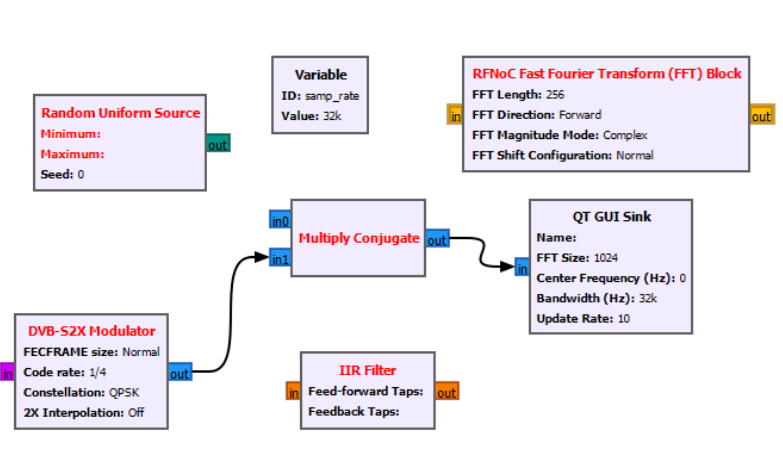
\includegraphics[width=\linewidth]{img/block-diagrams.png}
                 \caption{Blocks available}
                \label{fig:blocks_gnu}
            \end{figure}
        \end{column}
    \end{columns}
    % \begin{figure}
    %     \centering
    %     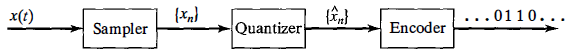
\includegraphics[width=0.7\linewidth]{img/PCM_steps.png}
    %     \caption{Block Diagram for a PCM System}
    %     \label{fig:enter-label}
    % \end{figure}
	
\end{frame}

%----------------------------------------------------------------------------------------
% \subsection{Sampling}\section{Resources}
\begin{frame}
	\frametitle{Resources}
    
\begin{columns}
        % First column
        \begin{column}{0.5\textwidth}
     \begin{itemize}
    \item Library with various processing blocks available in
    \begin{enumerate}
     \item Inside the GUI;
     \item C++;
     \item Python.
    \end{enumerate}
     \end{itemize}
     
        \end{column}
        
        % Second column
        \begin{column}{0.5\textwidth}
            \begin{figure}[t]
                \centering
                
\includegraphics[width=\linewidth]{img/GNU_radio_logo.png}
                 %\caption{Blocks Available}
                \label{fig:gnu_radio_logo}
            \end{figure}
            \begin{figure}
                \centering
                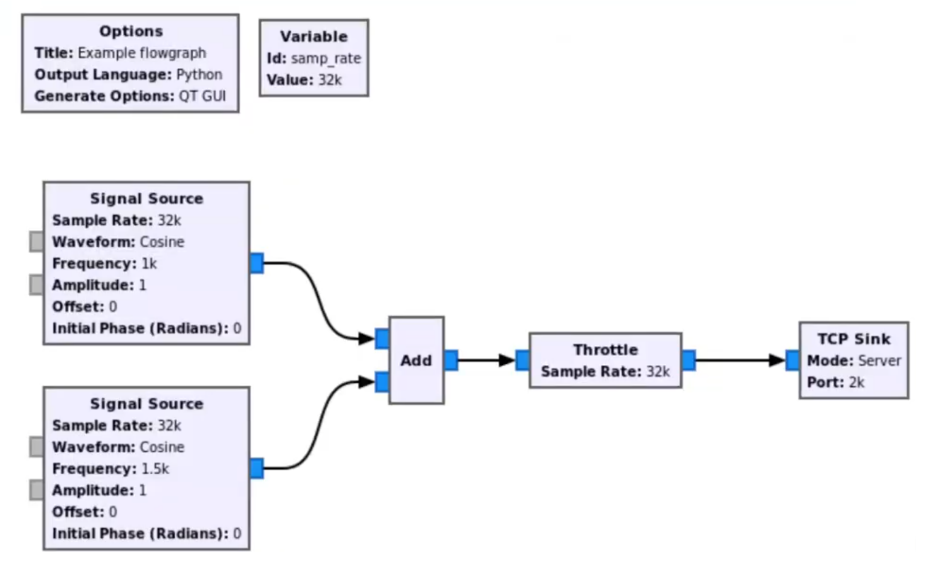
\includegraphics[width=\linewidth]{img/flowgraph example.png}
                 \caption{Flowgraph example}
                \label{fig:enter-label}
            \end{figure}
        \end{column}
    \end{columns}
    % \begin{figure}
    %     \centering
    %     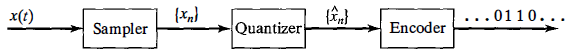
\includegraphics[width=0.7\linewidth]{img/PCM_steps.png}
    %     \caption{Block Diagram for a PCM System}
    %     \label{fig:enter-label}
    % \end{figure}
	
\end{frame}


%----------------------------------------------------------------------------------------

\begin{frame}
	\frametitle{Resources}
    
\begin{columns}
        % First column
        \begin{column}{0.5\textwidth}
     \begin{itemize}
    \item Library with various processing blocks available in
    \begin{enumerate}
     \item Inside the GUI;
     \item C++;
     \item Python.
    \end{enumerate}
     \end{itemize}
     
        \end{column}
        
        % Second column
        \begin{column}{0.5\textwidth}
            % \begin{figure}[t]
            %     \centering
            %     
\includegraphics[width=\linewidth]{img/GNU_radio_logo.png}
            %      %\caption{Blocks Available}
            %     \label{fig:gnu_radio_logo}
            % \end{figure}

 \begin{figure}
        \centering
        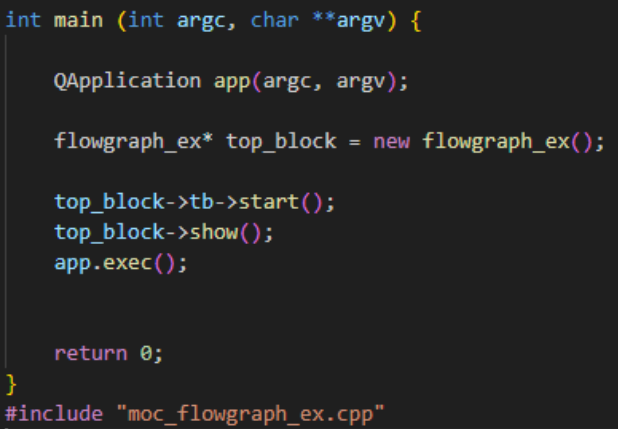
\includegraphics[width=0.5\linewidth]{img/c++.png}
        \caption{C++ output}
        \label{fig:enter-label}
    \end{figure}
                \begin{figure}
        \centering
        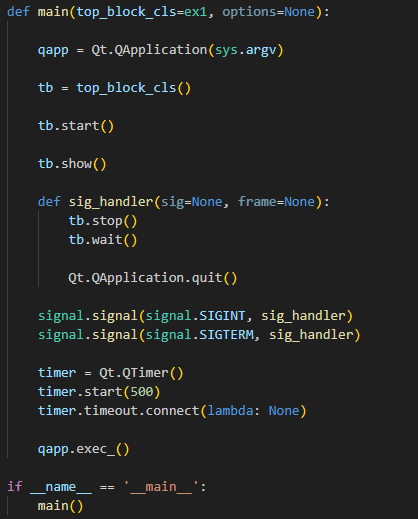
\includegraphics[width=0.3\linewidth]{img/python.png}
        \caption{Python output}
        \label{fig:enter-label}
    \end{figure}
            % \begin{figure}
            %     \centering
            %     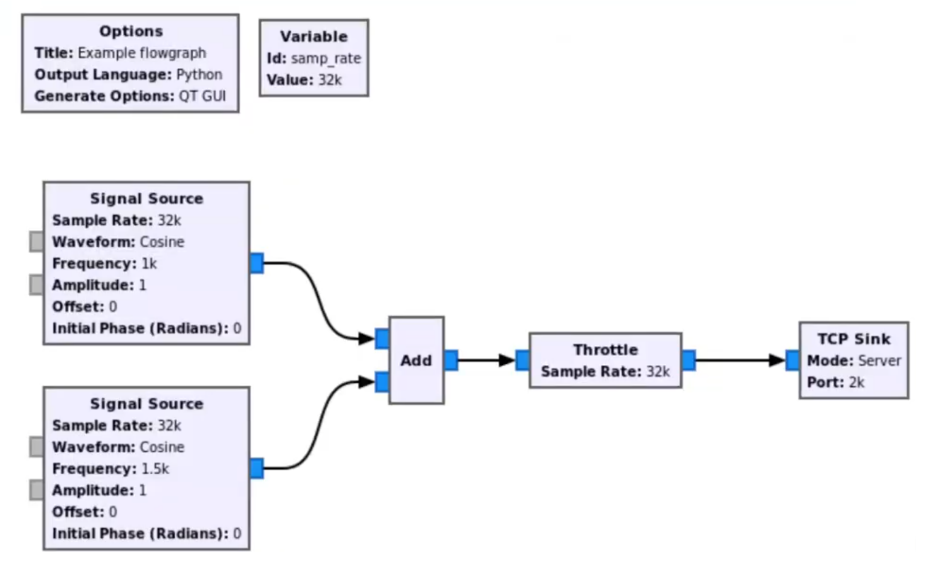
\includegraphics[width=\linewidth]{img/flowgraph example.png}
            %      \caption{Flowgraph example}
            %     \label{fig:enter-label}
            % \end{figure}
        \end{column}
    \end{columns}
    % \begin{figure}
    %     \centering
    %     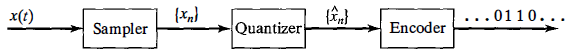
\includegraphics[width=0.7\linewidth]{img/PCM_steps.png}
    %     \caption{Block Diagram for a PCM System}
    %     \label{fig:enter-label}
    % \end{figure}
	
\end{frame}


%----------------------------------------------------------------------------------------

% \begin{frame}
% 	\frametitle{Resources}
    
% \begin{columns}
%         % First column
%         \begin{column}{0.5\textwidth}
   
%         \end{column}
        
%         % Second column
%         \begin{column}{0.5\textwidth}
         
%             % \begin{figure}
%             %     \centering
%             %     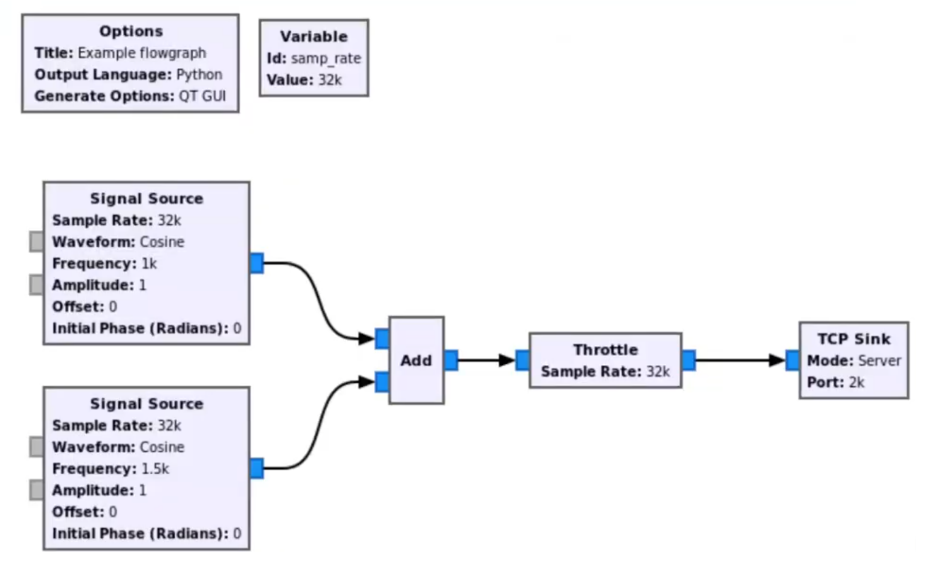
\includegraphics[width=\linewidth]{img/flowgraph example.png}
%             %      \caption{Flowgraph example}
%             %     \label{fig:enter-label}
%             % \end{figure}
%         \end{column}
%     \end{columns}
%     % \begin{figure}
%     %     \centering
%     %     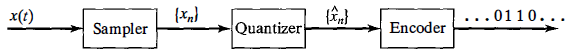
\includegraphics[width=0.7\linewidth]{img/PCM_steps.png}
%     %     \caption{Block Diagram for a PCM System}
%     %     \label{fig:enter-label}
%     % \end{figure}
	
% \end{frame}


%----------------------------------------------------------------------------------------



\section{Applications}
\begin{frame}
	\frametitle{Applications}
    
\begin{columns}
        % First column
        \begin{column}{0.5\textwidth}
     \begin{itemize}
    \item Defense and Security:
    \begin{enumerate}
    \item Signal intelligence and wireless security assessments;
    \item RF jamming detection and countermeasure development;
    \end{enumerate}
     \end{itemize}
     
        \end{column}
        
        % Second column
        \begin{column}{0.5\textwidth}
            \begin{figure}[]
                \centering
                
\includegraphics[width=\linewidth]{img/GNU_radio_logo.png}
                 %\caption{Blocks Available}
                \label{fig:gnu_radio_logo}
            \end{figure}
            \begin{figure}
                \centering
                
\includegraphics[width=0.5\linewidth]{img/applications/intelligence.png}
                %\caption{Defense}
                \label{fig:enter-label}
            \end{figure}
        \end{column}
    \end{columns}
\end{frame}

%----------------------------------------------------------------------------------------
%\subsection{Encoding}
%\section{Applications}
\begin{frame}
	\frametitle{Applications}
    
\begin{columns}
        % First column
        \begin{column}{0.5\textwidth}
     \begin{itemize}
    \item Telecommunications:
    \begin{enumerate}
     \item 5G and IoT prototyping and testing wireless communication protocols;
     \item Dynamic spectrum access and cognitive radio development.
    \end{enumerate}

     \end{itemize}
     
        \end{column}
        
        % Second column
        \begin{column}{0.5\textwidth}
            \begin{figure}[]
                \centering
                
\includegraphics[width=\linewidth]{img/GNU_radio_logo.png}
                 %\caption{Blocks Available}
                \label{fig:gnu_radio_logo}
            \end{figure}
            \begin{figure}
                \centering
                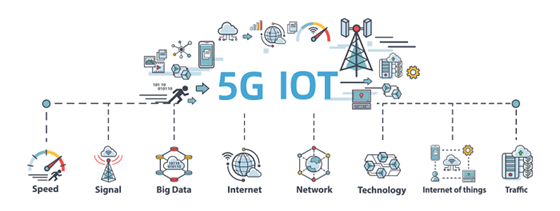
\includegraphics[width=\linewidth]{img/iot_5g.png}
                %\caption{Caption}
                \label{fig:enter-label}
            \end{figure}
        \end{column}
    \end{columns}
\end{frame}

%----------------------------------------------------------------------------------------

\begin{frame}
	\frametitle{Applications}
    
\begin{columns}
        % First column
        \begin{column}{0.5\textwidth}
     \begin{itemize}
    \item Satellite Communication:
    \begin{enumerate}
        \item Decoding telemetry and data from satellites including Cubesas and weather satellites.
        \item Supports ground station operations and satellite tracking.
    \end{enumerate}
     \end{itemize}
     
        \end{column}
        
        % Second column
        \begin{column}{0.5\textwidth}
            \begin{figure}[]
                \centering
                
\includegraphics[width=\linewidth]{img/GNU_radio_logo.png}
                 %\caption{Blocks Available}
                \label{fig:gnu_radio_logo}
            \end{figure}
            \begin{figure}
                \centering
                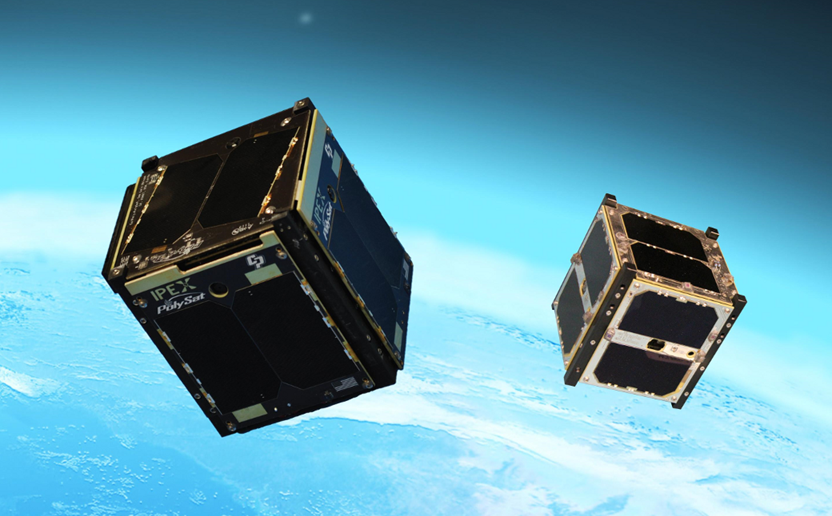
\includegraphics[width=\linewidth]{img/applications/satellite.png}
                %\caption{Caption}
                \label{fig:enter-label}
            \end{figure}
        \end{column}
    \end{columns}
\end{frame}

%----------------------------------------------------------------------------------------
%\section{Applications}
\begin{frame}
	\frametitle{Applications}
    
\begin{columns}
        % First column
        \begin{column}{0.5\textwidth}
     \begin{itemize}
    \item Academic and Research:
    \begin{enumerate}
        \item Lectures on Digital Signal Processing (DSP) and communication Systems.
        \item Valuable tool for prototyping new algorithms and conducting experiments on (RF) systems.
    \end{enumerate}
     \end{itemize}
     
        \end{column}
        
        % Second column
        \begin{column}{0.5\textwidth}
            \begin{figure}[]
                \centering
                
\includegraphics[width=\linewidth]{img/GNU_radio_logo.png}
                 %\caption{Blocks Available}
                \label{fig:gnu_radio_logo}
            \end{figure}
            \begin{figure}
                \centering
                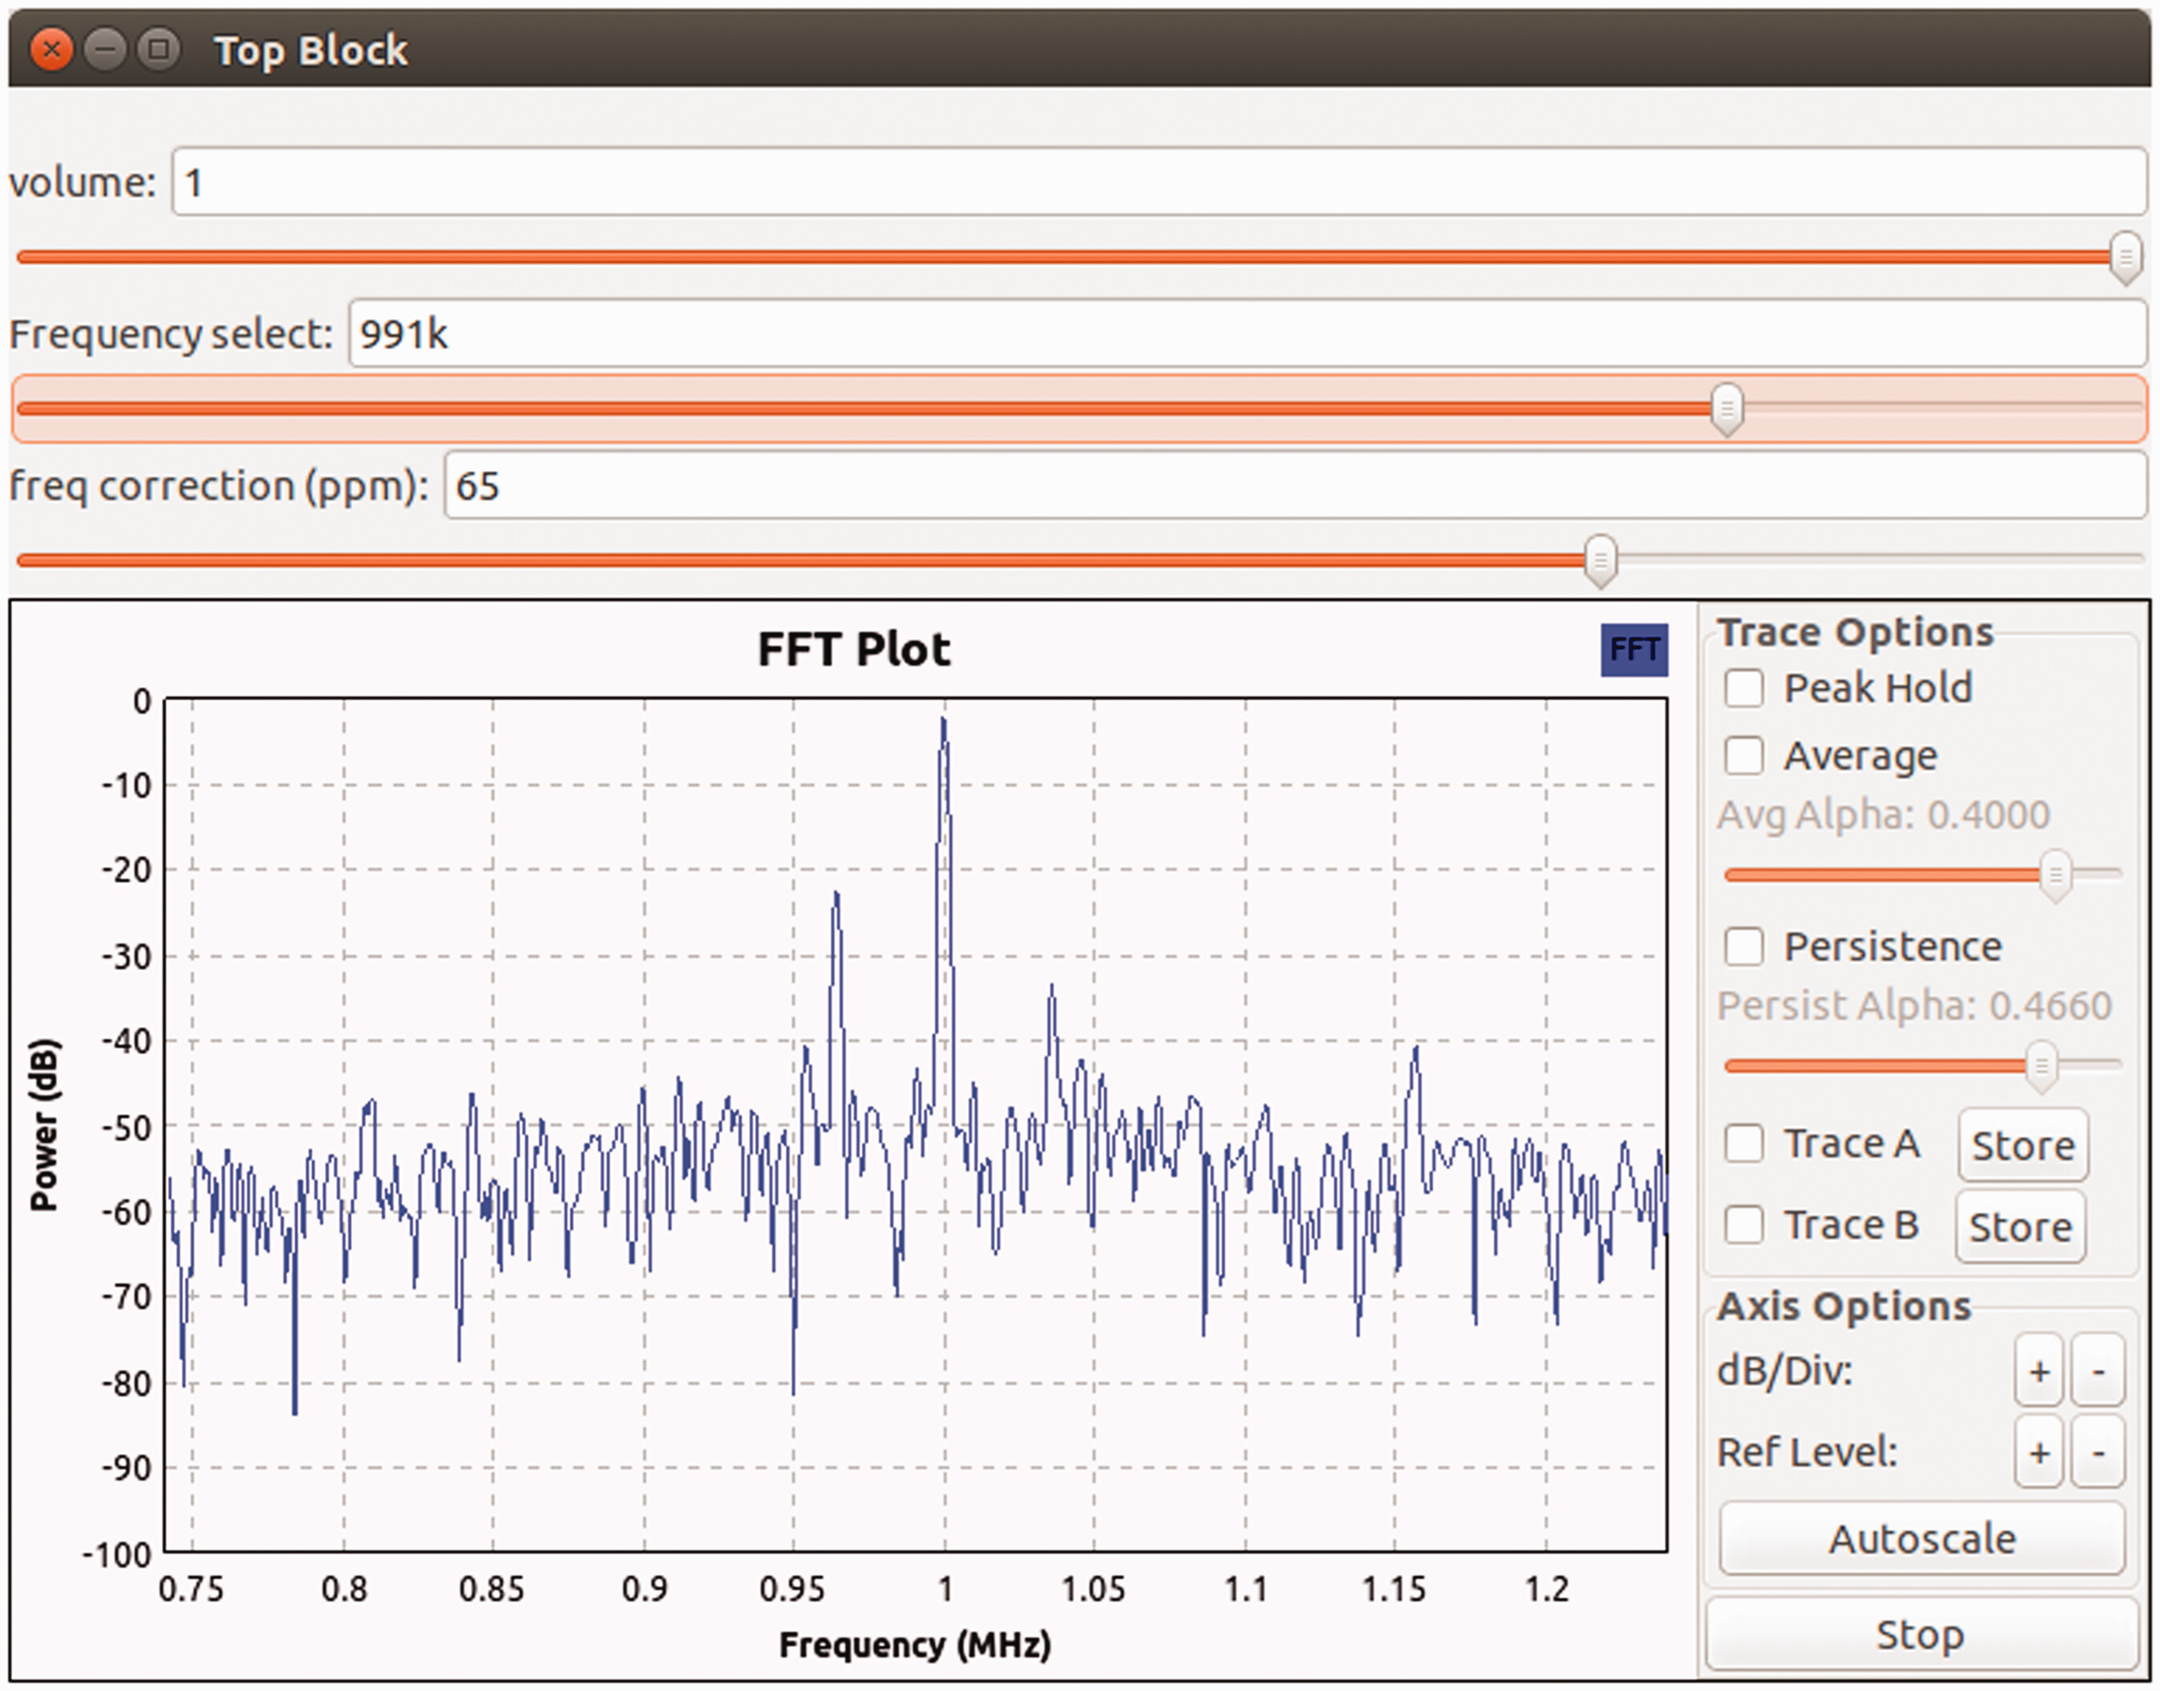
\includegraphics[width=.7\linewidth]{img/applications/learning.png}
                %\caption{Caption}
                \label{fig:enter-label}
            \end{figure}
        \end{column}
    \end{columns}
\end{frame}

%----------------------------------------------------------------------------------------
%\section{Applications}
\section{Practise}
\begin{frame}
	\frametitle{First Exercise}
    
\begin{figure}
    \centering
    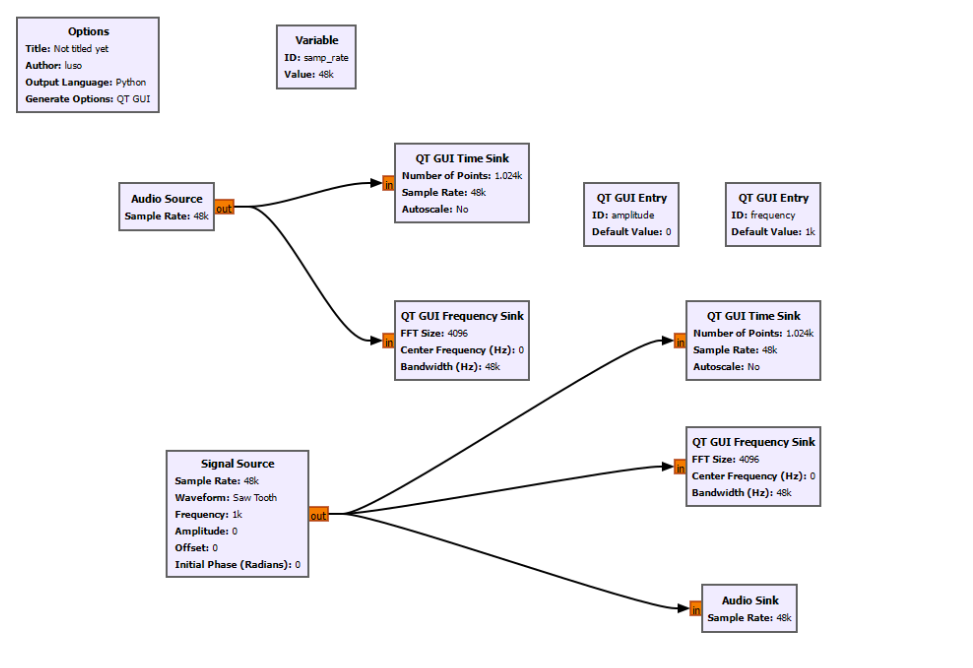
\includegraphics[width=0.8\linewidth]{img/applications/primeiro exercicio.png}
   % \caption{Caption}
    \label{fig:enter-label}
\end{figure}
\end{frame}
